\chapter{BCS theory}
\label{Ch_2}
\textit{Bardeen--Cooper--Schrieffer (BCS) theory} provides the first microscopic explanation: 
electrons near the Fermi surface form correlated pairs (\textit{Cooper pairs}) that behave effectively as \emph{bosons} and condense into a single macroscopic quantum state. 
\begin{center}
\textit{But electrons repel, how can they pair?}    
\end{center}


\section{Electron-Phonon interaction}
In a metal, electrons interact not only with each other through the Coulomb potential but also with the underlying ionic lattice.
Phonons provide a mechanism through which two electrons can experience an \textit{effective attraction}, despite their mutual repulsion.
This indirect, phonon-mediated attraction constitutes the microscopic origin of pairing in \textit{conventional superconductors}\footnote{Namely those materials that are accurately described by the BCS theory based on electron–phonon coupling.}.\\
By contrast, \emph{unconventional superconductors} (including cuprates, heavy-fermion compounds and some organic materials) cannot be explained solely by phonon-mediated pairing.\footnote{%
Their pairing mechanism likely arises from purely electronic interactions such as spin or charge fluctuations, and their superconducting order parameters often exhibit anisotropic or sign-changing symmetries.%
}

\subsection*{Physical mechanism}
When an electron moves through the crystal lattice, its negative charge slightly attracts the positively charged ions, producing a local distortion of the lattice potential.  
Because the ions are much heavier than the electrons, this deformation relaxes slowly compared to electronic motion.  \\
As the electron passes, the surrounding ions shift slightly towards it. Even after the electron has moved away, the ions relax slowly, producing a temporary region of excess positive charge.
A second electron traveling through the lattice can then be attracted to this residual distortion, effectively feeling a potential well created by the first electron.  
In this way, one electron polarizes the lattice, and another electron is drawn towards this polarization field: the two interact indirectly through the exchange of a \emph{virtual phonon}.  

\begin{figure}[H]
    \centering
    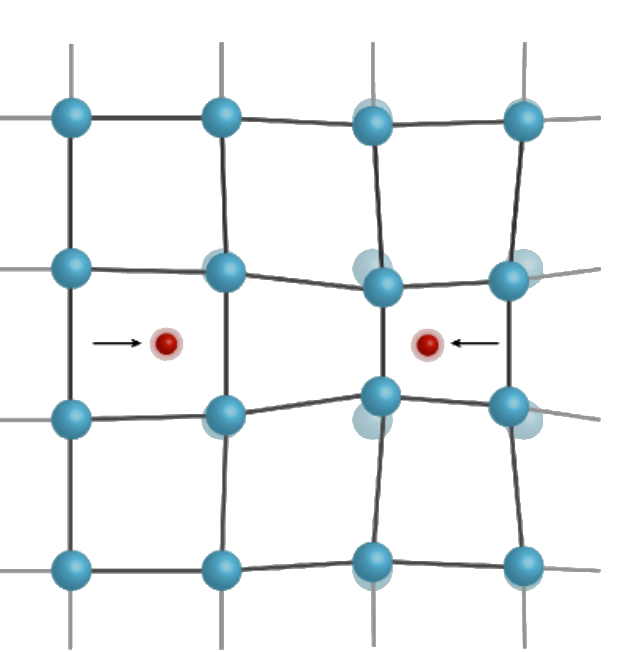
\includegraphics[scale = 0.65]{Chapters/Chapter_3/Images/3_phonon_mediated.png}
    \caption{Schematic representation of the phonon-mediated electron--electron attraction.
    As an electron moves through the lattice, it locally attracts the positively charged ions, creating a distortion that attracts a second electron.}
    \label{fig:phonon_mediated}
\end{figure}

This phonon-mediated process gives rise to an \textit{effective attractive interaction} between electrons, which can overcome their natural Coulomb repulsion under suitable conditions.

\section{Cooper Instability}
Having established that the electron–phonon interaction provides an effective attraction between electrons in a metal, we now turn to its microscopic consequences.\\
Two natural questions arise:

\begin{center}
\textit{Can such an attraction, weak as it may be, lead to the formation of bound states within the Fermi sea?}
\end{center}

and, if so,

\begin{center}
\textit{How does this affect the stability of the normal metallic ground state?}
\end{center}

To address these questions, we begin by considering the simplest possible system: a single pair of electrons interacting through an attractive potential, first in vacuum and then in the presence of a filled Fermi sea.\\
To this end, we first analyze the general two-body interaction problem through the Schrödinger equation, which will form the foundation for the discussion that follows.


\subsection*{Single Cooper Pair}
We begin by studying two electrons interacting via an attractive potential $V(\mathbf{r}_1-\mathbf{r}_2)$, and later apply these results to the cases of vacuum and of a filled Fermi sea.

Consider two electrons interacting via an attractive potential $V(\mathbf{r}_1-\mathbf{r}_2)$.
The two–body Schr\"odinger equation reads:
\begin{equation}
\left[
-\frac{\hbar^2\nabla_{\mathbf{r}_1}^2}{2m}
-\frac{\hbar^2\nabla_{\mathbf{r}_2}^2}{2m}
+ V(\mathbf{r}_1-\mathbf{r}_2)
\right]
\Psi(\mathbf{r}_1,\mathbf{r}_2)
= E\,\Psi(\mathbf{r}_1,\mathbf{r}_2).
\label{eq:cooper_sch}
\end{equation}
Introduce the \textit{centre-of-mass} (COM) and \textit{relative} coordinates as:
\[
\mathbf{R} = \frac{\mathbf{r}_1 + \mathbf{r}_2}{2},
\qquad
\mathbf{r} = \mathbf{r}_1 - \mathbf{r}_2.
\]
In these new variables, the Schrödinger equation~\eqref{eq:cooper_sch} becomes:
\begin{equation}
\left[
-\frac{\hbar^2\nabla_{\mathbf{R}}^2}{2M}
-\frac{\hbar^2\nabla_{\mathbf{r}}^2}{2\mu}
+ V(\mathbf{r})
\right]
\Psi(\mathbf{r},\mathbf{R})
= E\,\Psi(\mathbf{r},\mathbf{R}),
\label{eq:cooper_cm_sch}
\end{equation}
where \(M = 2m\) is the total mass and \(\mu  = m/2\) the reduced mass of the two-electron system.\\
Since the potential depends only on the relative coordinate \(\mathbf{r}\), the COM motion separates from the internal motion.  
We therefore make the ansatz:
\[
\Psi(\mathbf{r},\mathbf{R}) = \psi(\mathbf{r})\, e^{i\mathbf{K}\cdot\mathbf{R}},
\]
where \(\mathbf{K}\) is the total momentum of the pair and \(\psi(\mathbf{r})\) describes the internal structure of the bound state.  
Substituting this form into Eq.~\eqref{eq:cooper_cm_sch} yields the Schrödinger equation for the relative motion:
\begin{equation}
\left[
-\frac{\hbar^2\nabla_{\mathbf{r}}^2}{2\mu}
+ V(\mathbf{r})
\right]\psi(\mathbf{r})
= \tilde{E}\,\psi(\mathbf{r}),
\qquad
\tilde{E} = E - \frac{\hbar^2K^2}{2M}.
\label{eq:cooper_relative_sch}
\end{equation}
where:
\begin{itemize}
    \item \(E\) is the total energy of the two-electron system;
    \item \(\tilde{E} = E_{\mathrm{rel}}\) is the internal (relative-motion) energy associated with the pair’s binding;
    \item \(E_{\mathrm{COM}} = \hbar^2 K^2 / (2M)\) is the kinetic energy of the pair’s centre-of-mass motion, with \(M = 2m\) total mass.
\end{itemize}
The lowest-energy configuration corresponds to $\mathbf{K}=0$, where the total momentum of the pair vanishes and the two electrons have equal and opposite momenta.\\
Depending on the symmetry of the spatial wavefunction, different spin configurations arise in order to preserve the antisymmetry of the total fermionic wavefunction:
\begin{itemize}
    \item If the spatial part is \textit{even}, satisfying $\psi(\mathbf{r}) = \psi(-\mathbf{r})$,  
    the spin part must be \textit{antisymmetric}, corresponding to a \emph{singlet state}:
    \[
    \frac{1}{\sqrt{2}}\left(|\uparrow\downarrow\rangle - |\downarrow\uparrow\rangle\right).
    \]

    \item If the spatial part is \textit{odd}, satisfying $\psi(\mathbf{r}) = -\psi(-\mathbf{r})$,  
    the spin part must be \textit{symmetric}, forming a \emph{triplet state} with three possible spin projections:
    \[
    |\uparrow\uparrow\rangle, \quad
    |\downarrow\downarrow\rangle, \quad
    \frac{1}{\sqrt{2}}\left(|\uparrow\downarrow\rangle + |\downarrow\uparrow\rangle\right).
    \]
\end{itemize}
In conventional superconductors, pairing occurs in the singlet channel, corresponding to even spatial symmetry and opposite spins.

\paragraph{Fourier–space formulation}
To analyse the two-electron bound state it is convenient to work in momentum space.  
Fourier-transforming the relative-coordinate Schr\"odinger equation:
\[
\left[-\frac{\hbar^2\nabla_{\mathbf r}^2}{2\mu}+V(\mathbf r)\right]\psi(\mathbf r)
=\tilde E\,\psi(\mathbf r),
%\label{eq:cooper_relative_sch}
\]
one obtains at the Cooper Integral Equation\footnote{For a full derivation of the Cooper integral equation see Appendix~\ref{app:BCS-derivation}, section \ref{app:cooper_FT}.}:
\begin{equation}
\boxed{
\bigl(\tilde E-2\varepsilon_{\mathbf k}\bigr)\,\psi(\mathbf k)
=\int\!\frac{d^3 k'}{(2\pi)^3}\, V(\mathbf k-\mathbf k')\,\psi(\mathbf k')}\,,
\qquad
\varepsilon_{\mathbf k}=\frac{\hbar^2 k^2}{2m},
\label{eq:cooper_integral_body}
\end{equation}
where the kinetic term becomes diagonal and the interaction appears as a convolution in momentum space.
It is convenient to define:
\[
\Delta(\mathbf k)\equiv \bigl(E-2\varepsilon_{\mathbf k}\bigr)\,\psi(\mathbf k),
\qquad (E\equiv \tilde E\ \text{for }\mathbf K=0),
\]
which yields the compact homogeneous form:
\begin{equation}
\boxed{
\Delta(\mathbf k) = -\!\int\!\frac{d^3 k'}{(2\pi)^3}\;
\frac{V(\mathbf k-\mathbf k')}{\,2\varepsilon_{\mathbf k'}-E\,}\;\Delta(\mathbf k') } \,.
\label{eq:cooper_Delta_body}
\end{equation}
A nontrivial solution $\Delta(\mathbf{k}) \neq 0$ exists only for discrete energies satisfying $E < 2\varepsilon_{\mathbf{k}}$, corresponding to a bound state.
This condition reflects that the total energy of the two interacting electrons is lower than the energy of two independent free electrons, indicating the formation of a stable pair.\\
Thus, the phonon-mediated attraction between electrons therefore provides a microscopic mechanism capable of overcoming their natural Coulomb repulsion.  
%To understand the physical consequences of such an effective interaction, we now turn to the simplest possible system: a single pair of electrons interacting attractively.  
%By solving this two-body problem, we will uncover the essential physics of pairing and establish the foundation for the many-body BCS theory.

\subsection*{Cooper Pair Binding}

We now approach the problem of electron–electron pairing in two steps.  
First, we examine whether a bound state between two electrons can exist in \emph{vacuum} under an attractive interaction.  
Then, we embed the same two-body system in a \emph{metallic environment} (a Fermi sea\footnote{The \textit{Fermi sea} denotes the filled set of single-particle quantum states occupied by fermions up to the Fermi energy \(E_F\) at zero temperature.  
It represents the ground state of a noninteracting Fermi gas, in which all momentum states with \(|\mathbf{k}| \leq k_F\) are occupied, and those above \(k_F\) are empty.  
Excitations or interactions near the Fermi surface (\(|\mathbf{k}| = k_F\)) govern the low-temperature properties of metals and superconductors.%
} of occupied electronic states) and show that this dramatically changes the outcome, leading to what is known as the \textit{Cooper instability}.  

\paragraph{Two-Electron Bound State in Vacuum.}
We first consider the simplest case: two electrons in free space interacting through an effective attractive potential. Our goal is to determine whether such an interaction can lead to the formation of a bound state between the two fermions. We look for an even-parity solution of the relative wavefunction, \(\psi(\mathbf{r}) = \psi(-\mathbf{r})\), which corresponds to antiparallel electron spins and therefore a singlet configuration.  \\
In this scenario, the interaction is modelled in momentum space as a short-ranged potential acting only within a finite energy cutoff defined by the characteristic phonon frequency:
\[
V(\mathbf{k}-\mathbf{k}') =
\begin{cases}
    -V_0 & \text{if } \varepsilon_{\mathbf{k}},\,\varepsilon_{\mathbf{k}'} < \hbar\omega_D,\\[6pt]
    0 & \text{otherwise},
\end{cases}
%\label{eq:V_debye_shell_vac}
\]
where \(V_0 > 0\) measures the strength of the effective attraction and \(\hbar\omega_D\) denotes the Debye energy\footnote{%
The Debye energy \(\hbar\omega_D\) represents the maximum phonon energy in the Debye model of a solid, corresponding to the highest lattice vibrational mode.  
}, corresponding to the maximum phonon energy in the lattice. In this vacuum setting the cutoff simply restricts the interaction to low–energy states:
only single–particle modes with $\varepsilon_{\mathbf k},\varepsilon_{\mathbf k'}<\hbar\omega_D$ contribute, i.e.\ the potential is short–ranged in energy and does not involve high–energy states.\\
Since the potential is constant within the cutoff, the pair wavefunction in momentum space can also be taken as approximately constant, \(\Delta(\mathbf{k}) \simeq \Delta\).  
The integral equation for the two-particle bound state [Eq.~\eqref{eq:cooper_Delta_body}] then reduces to
\[
\Delta = V_0\,\Delta
\int_{\varepsilon_{\mathbf{k}'}<\hbar\omega_D}
\frac{d^3k'}{(2\pi)^3}\, \frac{1}{2\varepsilon_{\mathbf{k}'} - E}.
\]
Because a bound state requires \(\Delta \neq 0\), we can divide both sides by \(\Delta\), yielding
\[
1 = V_0
\int_{\varepsilon_{\mathbf{k}'} < \hbar\omega_D}
\frac{d^3k'}{(2\pi)^3}\,
\frac{1}{2\varepsilon_{\mathbf{k}'} - E},
%\label{eq:self_consistency_vacuum}
\]
where \(E < 0\) denotes the total energy of the pair.  
We now express the momentum integral in terms of the single-particle energy \(\varepsilon\)
using the density of states per spin:
\[
\rho(\varepsilon) =
\frac{1}{4\pi^2}
\left(\frac{2m}{\hbar^2}\right)^{3/2}\!\sqrt{\varepsilon}.
\]
This substitution transforms the integral over momentum space into one over energy:
\[
\int_{\varepsilon_{\mathbf k'}<\hbar\omega_D}
\frac{d^3k'}{(2\pi)^3}
\quad \rightarrow \quad 
\int_0^{\hbar\omega_D} \rho(\varepsilon)\, d\varepsilon,
\]
Thus the Cooper equation becomes
\begin{equation}
\boxed{
1 = V_0 \int_0^{\hbar\omega_D}
\frac{\rho(\varepsilon)\, d\varepsilon}{2\varepsilon - E}}
\label{eq:self_consistency}
\end{equation}
Equation~\eqref{eq:self_consistency} is the \textit{self-consistency condition} for the bound-state energy \(E\):
it expresses the requirement that a nontrivial solution (\(\Delta \neq 0\)) of the Cooper equation
can exist only for specific combinations of the interaction strength \(V_0\) and energy \(E\).\\
Evaluating the integral explicitly:
\[
\int_0^{\hbar\omega_D}\!\!\frac{\sqrt{\varepsilon}\,d\varepsilon}{2\varepsilon - E}
=
\left[
\sqrt{\hbar\omega_D}
- \sqrt{-\frac{E}{2}}\,
\arctan\!\left(\sqrt{\frac{2\hbar\omega_D}{-E}}\right)
\right],
\]
we obtain
\[
1 = V_0\,\frac{1}{4\pi^2}
\left(\frac{2m}{\hbar^2}\right)^{3/2}
\left[
\sqrt{\hbar\omega_D}
- \sqrt{-\frac{E}{2}}\,
\arctan\!\left(\sqrt{\frac{2\hbar\omega_D}{-E}}\right)
\right].
%\label{eq:self_consistency_result}
\]

The right-hand side depends explicitly on the bound-state energy \(E<0\).  
A nontrivial solution exists only if the attractive potential \(V_0\) exceeds a critical threshold.  
Setting \(E \to 0^{-}\) gives the limiting condition:
\begin{equation}
\boxed{
V_{0,\text{min}} = 4\pi^2
\left(\frac{\hbar^2}{2m}\right)^{3/2}
\frac{1}{\sqrt{\hbar\omega_D}}
= \frac{\sqrt{2}\,\pi^2\hbar^3}{m^{3/2}\sqrt{\hbar\omega_D}}}\,.
\label{eq:V0min}
\end{equation}

Hence, in vacuum, a bound state forms only when the attraction is strong enough, \[V_0 > V_{0,\mathrm{min}}.\]  
%This represents the usual molecular binding condition in free space.

\paragraph{Cooper Pairs in a Metal.}
We now place the same two electrons in a \emph{metallic environment}, where all single-particle states are filled up to the Fermi energy \(\varepsilon_F\). In a real metal, only electrons lying close to the Fermi energy are affected by the attractive interaction.
Therefore, the integration range in Eq.~\eqref{eq:self_consistency} is restricted to the \emph{Debye shell},
\(\varepsilon_F < \varepsilon < \varepsilon_F + \hbar\omega_D\),
which contains the electronic states coupled by phonons.
Within this narrow window, the density of states can be approximated by its value at the Fermi level, \(\rho(\varepsilon) \simeq \rho(\varepsilon_F)\), since \(\hbar\omega_D \ll \varepsilon_F\). Only those electrons close to the Fermi surface can participate in the interaction, since phonons couple electronic states within a narrow energy window of width \(\hbar\omega_D\).\\
Thus, we obtain:
\[
1 = V_0\,\rho(\varepsilon_F)
\int_{\varepsilon_F}^{\varepsilon_F+\hbar\omega_D}
\frac{d\varepsilon}{2\varepsilon - E}.
\]
Performing the integration yields
\begin{equation}
\frac{2}{V_0\rho(\varepsilon_F)} =
\ln\!\left(
\frac{2\varepsilon_F - E + 2\hbar\omega_D}{2\varepsilon_F - E}
\right).
\label{eq:cooper_log}
\end{equation}

To express this in terms of the binding energy, we define:
\[
E_b = 2\varepsilon_F - E,
\]
which measures how far the bound-state energy lies below the Fermi level.
Substituting into Eq.~\eqref{eq:cooper_log} gives:
\begin{equation}
\frac{2}{V_0\,\rho(\varepsilon_F)} =
\ln\!\left(\frac{E_b + 2\hbar\omega_D}{E_b}\right).
\label{0123}
\end{equation}
We now make a key assumption at the core of the BCS model: the system is in the \textit{weak-coupling limit}, and we seek non-perturbative solutions in this regime.  
This condition entails:
\begin{itemize}
    \item \(V_0 \rho(\varepsilon_F) \ll 1\), meaning that the effective attractive interaction between electrons is very small compared to the characteristic Fermi energy scale;
    \item Cooper pairs are highly delocalized in real space, with strongly overlapping wavefunctions and weak binding between the constituent electrons.
\end{itemize}
Consequently, the binding energy \(E_b = 2\varepsilon_F - E\) is much smaller than the phonon cutoff energy, \(E_b \ll \hbar\omega_D\).  
In this regime, the logarithm in Eq.\eqref{0123} can be approximated by its dominant term,
\[
\ln\!\left(\frac{E_b + 2\hbar\omega_D}{E_b}\right)
\simeq
\ln\!\left(\frac{2\hbar\omega_D}{E_b}\right),
\]
since the correction proportional to \(E_b\) is negligible. Substituting this approximation back into Eq.~\eqref{0123} yields:
\[
\frac{2}{V_0\rho(\varepsilon_F)}
\simeq
\ln\!\left(\frac{2\hbar\omega_D}{E_b}\right),
\]
which can be inverted to obtain the \emph{binding energy}:
\begin{equation}
\boxed{
E_b = 2\hbar\omega_D\,e^{-\tfrac{2}{V_0\, \rho(\varepsilon_F)}}}\, .
\label{eq:Eb_final}
\end{equation}
\noindent
This result has a profound implication: a bound state can form between two electrons
\emph{for any arbitrarily small attractive potential} (\(V < 0\)).
Such a bound state is known as a \emph{Cooper pair}.
This behaviour contrasts sharply with the free-electron case in vacuum,
where the attractive interaction must exceed a finite threshold to produce a bound state.

In a metal, however, the presence of a well-defined Fermi surface fundamentally changes the situation:
it separates occupied from unoccupied electronic states, creating the conditions under which
even an infinitesimal attraction can lead to the formation of a bound pair.
The existence of this bound state marks the first step towards understanding
the microscopic origin of superconductivity.



%TO DO!! Check whether put it or not

\begin{comment}
\paragraph{Finite momentum and supercurrent}
For a pair with finite centre-of-mass momentum \(\mathbf{K}\), the total energy reads:
\begin{equation}
E = 2\varepsilon_F - E_b + \frac{\hbar^2 K^2}{4m}.
\end{equation}
Thus, in the limit $E \to 2 \varepsilon_F$, the corresponding centre-of-mass momentum and associated current density are:
\begin{equation}
K = \frac{2}{\hbar}\sqrt{mE_b}, 
\qquad
J = n_s e\frac{\hbar K}{m}
= 2n_s e\sqrt{\frac{E_b}{m}},
\end{equation}
where \(n_s\) is the density of superconducting pairs.
This expression connects the microscopic pairing mechanism to the macroscopic flow of supercurrent observed in superconductors.
\end{comment}

%============================== CHECK THIS SECTION ================================ %TO DO!!
\section{Many Cooper Pairs}

In the previous section, we showed that even a very weak attractive interaction can bind two electrons into a correlated pair.  
Such a pair carries total charge \(2e\) and, in the singlet case, total spin zero, so it behaves effectively as a boson.\\
A real superconductor, however, contains not just a single pair but an enormous number of electrons close to the Fermi surface.  
All these electrons experience the same effective attraction and form a highly overlapping collection of Cooper pairs that share a common quantum phase.  
The central idea of BCS theory is that these pairs do not exist as isolated molecules, but as a collective macroscopic quantum state.

In what follows, we will not delve into the full microscopic derivation, whose algebraic steps (mean-field decoupling, Bogoliubov transformation, self-consistency conditions) can be lengthy.
Instead, we present the essential physical picture that captures how a macroscopic number of overlapping Cooper pairs organize into the coherent condensate characteristic of the superconducting state.

\subsection*{Physical picture}

Electrons near the Fermi energy tend to form time-reversed pairs of the form 
\((\mathbf{k}\uparrow,-\mathbf{k}\downarrow)\): they have opposite momenta, opposite spins, and therefore zero total momentum.  
Because the effective attraction is weak, each pair is extremely extended in real space, with a size much larger than the average interparticle spacing.  
As a consequence, different Cooper pairs overlap strongly, and a single electron can simultaneously participate in many pairing configurations.

As will be discussed in the next chapter, a remarkable feature of this regime is that pairing and condensation are inseparable processes:
\[
\text{pair formation} \quad \Longleftrightarrow \quad \text{condensation at } T_c.
\]
The moment the effective attraction destabilizes the Fermi sea, a macroscopic number of overlapping pairs form and collectively lock into a single coherent quantum state.  
It is this collective behaviour, rather than the binding of isolated electron pairs, that gives rise to the superconducting phase.

\paragraph{BCS ground-state wavefunction}
The collective superconducting state is described by the BCS ground-state wavefunction.  
Instead of stating that each momentum state \(\mathbf{k}\) is either filled or empty, BCS theory assigns to it a quantum superposition of the two possibilities.  
The ground state is given by
\begin{equation}
|\Psi_{\mathrm{BCS}}\rangle =
\prod_{\mathbf{k}}
\bigl(u_{\mathbf{k}} + v_{\mathbf{k}}\,
c_{\mathbf{k}\uparrow}^{\dagger}c_{-\mathbf{k}\downarrow}^{\dagger}\bigr)
\,|0\rangle,
\qquad |u_{\mathbf{k}}|^2 + |v_{\mathbf{k}}|^2 = 1.
\label{BCS_groundstate}
\end{equation}

Here:
\begin{itemize}
    \item \(c_{\mathbf{k}\sigma}^{\dagger}\) creates an electron with momentum \(\mathbf{k}\) and spin \(\sigma\);
    \item \(c_{\mathbf{k}\uparrow}^{\dagger}c_{-\mathbf{k}\downarrow}^{\dagger}\) creates a Cooper pair with zero total momentum;
    \item \(u_{\mathbf{k}}\) and \(v_{\mathbf{k}}\) are the amplitudes for the pair state \((\mathbf{k},-\mathbf{k})\) to be empty or occupied;
    \item \(|0\rangle\) denotes the filled Fermi sea of the normal state.
\end{itemize}

Each factor \((u_{\mathbf{k}} + v_{\mathbf{k}} c_{\mathbf{k}\uparrow}^{\dagger}c_{-\mathbf{k}\downarrow}^{\dagger})\)  
represents a coherent superposition of “no pair in mode \(\mathbf{k}\)” and “one Cooper pair in mode \(\mathbf{k}\)”.  
The full superconducting ground state is the product of these contributions, forming a condensate of Cooper pairs all sharing the same global phase.

This structure makes the connection with Bose--Einstein condensation explicit:  
Cooper pairs with zero total momentum occupy a common coherent quantum state,  
but with a momentum-dependent weight \(v_{\mathbf{k}}\) rather than populating a single momentum mode.

\bigskip
Up to this point, we have established the microscopic mechanism responsible for the formation of Cooper pairs.\\  
However, the emergence of superconductivity as a macroscopic quantum phenomenon requires understanding how these pairs collectively condense into a coherent quantum state.  
To address this, in the next chapter we turn to the concept of \textit{Bose–Einstein condensation}, which describes the collective behaviour of these composite bosons.









\begin{comment}
%============================== CHECK THIS SECTION ================================ TO DO!!
%============================== CHECK THIS SECTION ================================
%============================== CHECK THIS SECTION ================================
\section{The BEC--BCS Crossover}
\label{sec:BEC-BCS-crossover}

The BCS and BEC descriptions represent two complementary limits of the same underlying phenomenon---the condensation of paired fermions.  
In the \emph{BCS limit}, the attraction between electrons is weak and their pairs are highly overlapping, forming a collective quantum state characterized by long-range phase coherence but little spatial localization.  
In the \emph{BEC limit}, the attraction becomes strong enough to form tightly bound pairs behaving as independent bosons that undergo Bose--Einstein condensation.  
Between these two limits lies a smooth, continuous evolution known as the \emph{BEC--BCS crossover}.

As the interaction strength increases, the \textit{pair size} $\xi_{\mathrm{pair}}$ gradually decreases from much larger than the average inter-particle spacing ($\xi_{\mathrm{pair}} \gg n^{-1/3}$) in the BCS regime, to much smaller than it ($\xi_{\mathrm{pair}} \ll n^{-1/3}$) in the BEC regime.  
Concurrently, the \textit{chemical potential} $\mu$ evolves from approximately the Fermi energy ($\mu \approx \varepsilon_F$) in the weak-coupling limit to negative values ($\mu \approx -E_b/2$) characteristic of bound molecules in the strong-coupling limit.  
Despite these microscopic changes, the transition is \emph{continuous}: there is no phase boundary separating BCS and BEC superconductivity.  
Both phases share the same broken $\mathrm{U}(1)$ gauge symmetry and are described by a common complex order parameter:
\[
\Delta = |\Delta|\,e^{i\phi},
\]
which reflects the global phase coherence of the condensate.\\
The unified picture is therefore that of a single condensate whose microscopic nature evolves smoothly with interaction strength:
\[
\text{BCS: overlapping pairs, }\mu > 0
\;\longleftrightarrow\;
\text{BEC: bound molecules, }\mu < 0.
\]
In real materials, such as high-$T_c$ cuprates or ultracold Fermi gases, the physical regime often lies in between these two extremes.  
Here, pairing and condensation occur on comparable energy scales---a situation referred to as the \emph{intermediate-coupling regime}.  
This region is of particular interest because it combines the strong pairing tendency of the BEC side with the long-range coherence of the BCS side, potentially accounting for the enhanced critical temperatures observed experimentally.

\end{comment}